%----------------------------------------------------------------------------------------------
\newpage
\begin{savequote}[108mm]
 "Anyone who has never made a mistake has never tried anything new." 
  \qauthor{Albert Einstein}
\end{savequote}
\chapter{Introduction}
\vspace{-3cm}
\label{chap:introduction}
%----------------------------------------------------------------------------------------------
  \section{About this document}
  \label{sec:about}
  The focus of this study is to explore the challenges and solutions to the obstacles associated with the migration from proprietary to Free and Open Source Software. These challenges will be discussed in greater detail in subsequent chapters. The weight of the study supports the migration to Free and Open Source Software from proprietary software. However, in order to provide a balanced perspective, it is necessary to understand the advantages of proprietary software. One of the key advantages is that one has the use of the proprietary software company's customer service and support when a problem arises. This is an advantage in terms of convenience, but it often comes at a price. With proprietary software there is a single entity who is accountable and responsible for bugs and solutions to them. With Free and Open Source software, this might not be the case and the company may have to hire a consultant or develop a fix themselves.  

  Free and Open Source Software offers an inexpensive alternative to proprietary, at least from the point of view of purchasing. For this reason, many private and government entities are choosing to migrate their data from proprietary software to Free and Open Source Software.  At first, this may seem like the logical choice, but there are many hidden costs and obstacles that can hinder the migration process. 

  An exploration of phased migrations in many parts of the world found that having on-site support personnel resolved many of the training and technical issues that arose. This was the case in both Germany and Spain. In the Largo, Florida case, a thorough needs assessment played a role in the success of the migration efforts.

  Several factor had an impact on the success of the migration to Free and Open Source Software. These included: 
  \begin{itemize} [itemsep=0ex]
  \item Gaining a thorough understanding of the needs of the organization and developing 	a sufficient support strategy.
  \item The level of complexity of the project.
  \item Developing comprehensive short term, mid-range, and long term goals of the organization in terms of the migration process.
  \item The level of commitment of all parties involved.
  \end{itemize}
 
  Case studies have demonstrated that Free and Open Source Software can be a viable solution for government entities and that it represents good stewardship of public funds. Cases demonstrate that with proper planning, the migration process can be successful and result in a system that functions comparably to the proprietary system, but at a fraction of the cost. It is recommended that government entities should consider migration to Free and Open Source Software as a means to control costs. 

  \subsection{Motivation}

  The motivation for this project stems from my work as a software programmer. Through my course of study, I have become aware of the problems associated with proprietary software and with the robustness of Free and Open Source Software. The migration process represents some of the greatest obstacles to success. These challenges form the basic motivation for this research. Through solving these issues, it is my hope that I may be able to give back to my community and my country. 



  \subsection{Research method and timeline}

  This section describes the method used when writing this research, and the timeline:
\begin{enumerate}[itemsep=0ex]
  \item  First step (started in December 2013): collect and read as much information as possible about Free and Open Source Software and migration in particular.
  \item The second: involves selecting the information from various sources. Books, online documents/web pages, related literature.
  \item Third: construct a detailed plan of the thesis.
  \item Fourth: Initial writing, draft the various sections and compile sections into first draft of thesis. 
  \item Fifth: check the flow of the thesis, undertake any additional editing and research. 
  \item Final: final draft check for errors, prepare for submission proof-read  final editing, compile bibliography, get the thesis bound and submit the thesis in November 2014.
\end{enumerate}
 
The research period is from December 2013 to November 2014.. Figure~\ref{fig:planning} provide diagram of this work.

   \begin{figure}
    \centering
        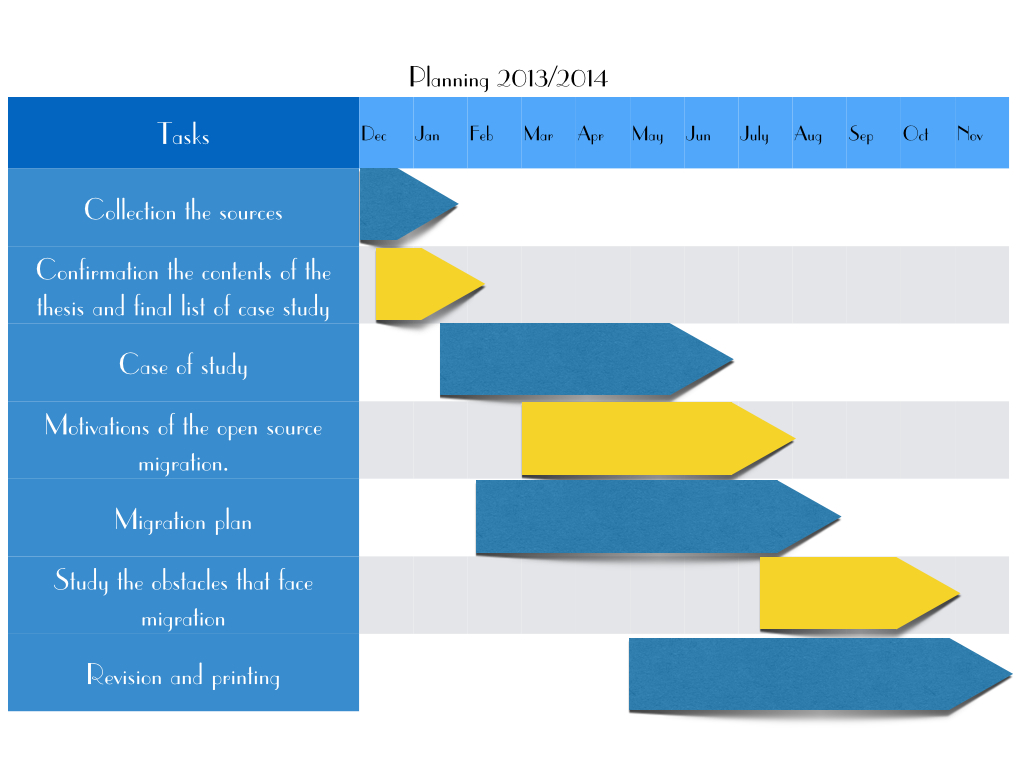
\includegraphics[scale=0.45]{img/planning.jpg}
      \caption{Work Plan and Timeline}
      \label{fig:planning}
    \end{figure}

In this thesis I've used quotes ('') and italic font to identify a direct quote. I've cited the original source in the footnote. I've used two methods of putting others ideas into my own words by paraphrasing and summarizing. The original source is shown in the Bibliography.
 %----------------------------------

\subsection{Structure of the thesis}

This document is divided into seven chapters. Chapter~\ref{chap:introduction} is the introduction. It explores the rationale behind the research and presents the motivation behind the research. Chapter~\ref{chap:Goals}  outlines the goals and objectives of the research. Chapter~\ref{chap:Motivations} supports the motivation for using Free and Open Source Software. Chapter~\ref{chap:plans} outlines a basic plan for migration to Free and Open Source Software from proprietary software.  Chapter~\ref{chap:Obstacles} outlines certain obstacles that may be encountered during the migration process. Chapter~\ref{chap:Caseofstudy}  presents several related case studies. Finally, conclusions are drawn in Chapter~\ref{chap:conclusions}, including lessons learned and future work.

 Wherever possible, the first time an abbreviation is used the expanded version will also be included in Appendix~\ref{apn:Acronyms}.
 
 %----------------------------------
 \section{Basic Concepts }

In order to facilitate a basic understanding of this work, the following terms are defined, ensuring that the reader will have a clear explanation of the concepts contained herein:
 
 \subsection{Free software}
 \label{sec:freeopen}
Free software, sometimes referred to as \emph{Libre software} are programs that, by default, include the necessary licensing at no additional charge to the user which allow the user to
 (i) run the program for any of the allowed purposes, (ii) study and modify the program, and (iii) to redistribute copies of either the original or modified program without having to pay any royalties to the software developers. The concept of free software was conceived by Richard Stallman in 1983 with the implementation of the \ac{GNU} Project. The \ac{FSF} \footnote{\url{http://www.fsf.org}}  was likewise subsequently created for the purpose of advocating for free software ideals as outlined in the Free Software Definition which states that free software means software that respects the user’s freedom and community. In essence, users have the freedom to run, copy, distribute, study, modify, and improve the software. A program is classified as free software if the program allows users the following four basic freedoms:

 \begin{enumerate}
 \item The freedom to run the program, for any (legal) purpose.
 \item The freedom to study how the program works, modifying it as desired.
 \item The freedom to redistribute copies without recompense to any individual or entity. 
 \item The freedom to distribute copies of the modified version to others without recompense to any individual or entity.
 \end{enumerate}

  \subsection{Open source}
 The open source movement is a worldwide movement consisting of individuals who believe that the best way to produce software that may be described as sophisticated, robust, and (for the most part) free of bugs is to enlist the cooperation of interested, skilled, and altruistic programmers, some of them professionals who work by appointment for high-tech companies, other volunteers who work on an altruistic manner. These individuals are inspired by the twin goals of producing high-quality programs and working cooperatively with other similarly minded individuals.
 \newline
 
Outline of Key Conditions of OSS Definition\footnote{By Feller and Fitzgerald in \url{http://www.brian-fitzgerald.com/wp-content/uploads/2011/07/open-source-icis00.pdf}}:
\textit{\begin{itemize}
\item The source code must be available to users.
\item The software must be redistributable.
\item The software must be modifiable and the creation of derivative works must be permitted.
\item The license must not discriminate against any user, group of users, or field of endeavor.
\item The license must apply to all parties to whom the software is distributed.
\item The license cannot restrict aggregations software.
 \end{itemize} }
 
 Thus it can be inferred from the above definitions and meaning that the Free and Open Source Software is the new and innovative software developed for the organizations and companies in order to meet the needs and requirements at challenging circumstances. The initiation and adoption of Free and Open Source Software in the companies and the organizations came into existence due to the improvement in the \ac{ICT}. The end users has all rights to edit and modify the codes of the software if possess the license.
 
  The term \ac{OSS} was adopted as an alternative term to ``free'' software given the fact that the term was not only less confusing, but that it worked to better describe the embodiment of the concept. The terms ``\textbf{open source software}'' and ``\textbf{free software}'' are typically used to describe the same programs, with the two terms often being used interchangeably. In fact, there are those who argue that the use of the two different terms, given their similarities, is simply one of a philosophical, rather than practical, difference between the two, and that the difference is primarily a matter of marketing as opposed to the actual substance of the two. Those who prefer to use the term ``\textbf{OSS}'' typically emphasize the technical advantages of the software that are present, such as the security of the program or the reliability of the program, while those who prefer the term ``\textbf{free software}'' tend to place their emphasis on the ethical issues addressed through the use of these types of software or the freedom from control of the developers or distributors that these types of programs offer\footnote{\url{http://www.osepa.eu/site pages/News/ 43/WhyOSS Look at the numbers Wheeler 2007.pdf}}. Regardless of perspective, it is important to note that the differences in these categories are extremely small, with almost all free software classified as open source software and almost all open source software as free software. 
 
 Other alternative terminology used to identify these types of programs includes:   \ac{OSS/FS}, \ac{FOSS} and  \ac{FLOSS}.  For the purpose of this thesis, \ac{FLOSS} is used to indicate that the software described has the characteristics that are implicit in both the terms ``open source software'' and ``free software''.

  \subsection{Other terms}
  The below terms are all associated with FLOSS in one way or another and some of them will be utilized throughout the course of this thesis. Figure~\ref{fig:categoriesofsoftware} shows the relationship present between these different types of software.
    %--------------------------------------------
     \subsection*{Copylefted software}
    Free software whose distribution terms work to ensure that all copies of all versions carry the same basic distribution terms.
       %--------------------------------------------
 \subsection*{Careware, also known as Charityware} 
Software that is licensed in such a way that it benefits a charity. There are several different types of careware in existence: free careware is completely free software; open source careware is free with the source code being made available to users, as in the case with text editor Vim\footnote{\url{http://www.vim.org/sponsor/}} which is free and OSS and is released under a license that includes some charityware clauses encouraging users who enjoy the software to consider donating to children in Uganda; and commercial careware, wherein the proceeds from the sale of the software are split between the developer and a supported charity. 
  %--------------------------------------------
         \begin{figure}[H]
             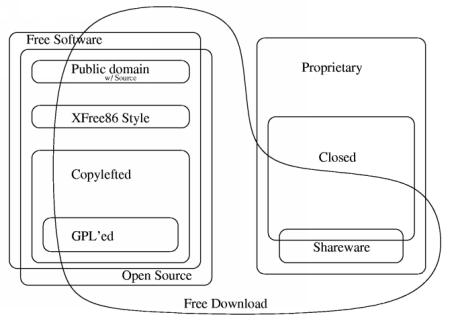
\includegraphics[scale=0.97]{img/free-open.jpg}
           \caption{Different Categories of Software (GNU.org, 2014)}
           \label{fig:categoriesofsoftware}
         \end{figure}

    \subsection*{Public domain software}
    Software that is completely free and may be used by any individual for any legal purpose. The software is not copyrighted as it has been donated to the public domain by the holder of copyright and is considered to be a part of the cultural heritage.
  %--------------------------------------------
    \subsection*{Proprietary software}
    The opposite of OSS, also known as \ac{CSS}. These types of software are licensed under the exclusive legal right of the copyright holder with the intent that the licensee is given the right to utilize the software only under specific conditions, with the restrictions on the use of the software typically enumerated in the  \ac{EULA}. Restrictions are placed on the use of the software, including the prevention of modification, sharing, studying, redistributing, and reverse engineering. In addition, the source code is not made available for common view.
       %--------------------------------------------
      \subsection*{Free software}
    A type of proprietary software copyrighted by the developer. The developer retains the rights to control the distribution, modification, and duration of time that the software is offered for use free of monetary charges. This software is typically distributed without its source code, making it differ from free software. 
%--------------------------------------------
  \subsection*{Shareware}
  Software that is provided to users, typically on a limited trial basis that restricts any and all commercial benefits, use, or exploitation of the software. It is distributed without an initial charge, but the user is strongly encouraged to pay a nominal fee for continued use.   

   %-------------------------------------------- 
   \subsection*{System migration}   
The act of physically transferring data and programs from an old system to a new system. This action is typically accomplished when the old hardware is no longer capable of meeting the needs of the user or when components have become damaged. This process may be simplified by the use of tools and software that allow for the automatic conversion of data up to and including the conversion of the code from one platform to another. 
 %----------------------------------------------------------------------------------------------
   \subsection*{Data migration}
   The process of transporting data between computers, storage devices, or from one format to another; an essential part of any system implementation, upgrade, or consolidation. During this process, software programs or scripts are utilized to map system data for automated migration. Ideally, data should be preserved when completing server or storage equipment replacements, when upgrading, consolidating websites, completing server maintenance, relocating between data centers, or when switching between application versions. Typically, this process requires converting the data into a suitable format for the new system, and it may become necessary to write a program that will automatically process the files being migrated from the old database, automatically inputting them in the new database, especially if the two are organized differently. 
   %----------------------------------------------------------------------------------------------

%-----------------------------------------------------------------------------------
      \cleardoublepage


      \begin{savequote}[108mm]
       ``Set your goals high, and don't stop till you get there.''
        \qauthor{ Bo Jackson}
      \end{savequote}

      \chapter{Goals and Objectives}
      \vspace{-3cm}
      \label{chap:Goals}



 %-----------------------------------------------------------------------------------------

\section{Goals} 

The primary goal of this research is to explore the FLOSS migration in government and private organizations. It is to gain as much knowledge as possible about the migration process so that the concepts learned by this study can be taken home and put into place. By examining the lessons learned by others, it is possible to avoid some of the pitfalls and to make the transition process as smooth as possible.          
                                                                                        
\section{Objectives}
Objectives allow the researcher to turn their concepts and ideals into a working plan. In order to achieve the goals that this research intends to accomplish, the following objectives will be met by this research:

\begin{enumerate}
\item To discover the main reasons why individuals, organizations, and companies are attracted to FLOSS. 
\item To examine the technical, economic, and social benefits of FLOSS.
\item To determine the best method for migration and implementation of FLOSS.
\item To develop a plan for successful migration to FLOSS that addresses the main areas of concern. Provide the main steps necessary for a successful migration.
\item To determine  the main obstacles that organizations face in the migration process.
\item To explore case studies that may provide clues as to the obstacles that the company will face and to explore some possible solutions through examining the experiences of others. and examine the total cost of migration in some cases.
\end{enumerate}
